\documentclass[11pt,a4paper]{article}

% --- Essential Packages ---
\usepackage[utf8]{inputenc}
\usepackage[margin=1in]{geometry}
\usepackage{amsmath,amssymb,amsthm,mathtools}
\usepackage{microtype}
\usepackage{booktabs}
\usepackage{enumitem}
\usepackage{xcolor}
\usepackage{tikz}
\usetikzlibrary{arrows.meta, positioning, shapes.geometric, calc}
\usepackage{tcolorbox}
\tcbuselibrary{skins,breakable}
\usepackage{hyperref}

% --- Color Palette (Subtle Academic / Deep Mind Palette) ---
\definecolor{primaryblue}{RGB}{24, 43, 73}
\definecolor{accentcrimson}{RGB}{140, 29, 64}
\definecolor{slateborder}{RGB}{203, 213, 225}
\definecolor{boxbg}{RGB}{248, 250, 252}
\definecolor{mathgray}{RGB}{71, 85, 105}

\hypersetup{
    colorlinks=true,
    linkcolor=primaryblue,
    citecolor=accentcrimson,
    urlcolor=primaryblue
}

% --- Custom Environments ---
\newtcolorbox{principlebox}[2][]{
    enhanced,
    colback=boxbg,
    colframe=primaryblue,
    fonttitle=\bfseries\sffamily\color{white},
    colbacktitle=primaryblue,
    title={#2},
    arc=3mm,
    boxrule=1pt,
    left=4mm, right=4mm, top=3mm, bottom=3mm,
    breakable,
    #1
}

\newtcolorbox{lawbox}[2][]{
    enhanced,
    colback=boxbg,
    colframe=accentcrimson,
    fonttitle=\bfseries\sffamily\color{white},
    colbacktitle=accentcrimson,
    title={#2},
    arc=3mm,
    boxrule=1pt,
    left=4mm, right=4mm, top=3mm, bottom=3mm,
    breakable,
    #1
}

\newtheorem{definition}{Definition}[section]
\newtheorem{theorem}{Theorem}[section]
\newtheorem{axiom}{Axiom}[section]

% --- Document Metadata ---
\title{\vspace{-1.5cm}\textbf{\huge The Symmetry-Invariant Metalearning System (SIMS)}\\[0.3em]
\Large\textit{A Category-Theoretic and Neurocomputational Framework for Accelerated Encoding, Dynamic Compression, and High-Transfer Problem Solving}}
\author{\textbf{Subham} \and \textbf{Antigravity Cognitive Systems Architecture}}
\date{Unified System Specification | Physics, Mathematics, and Cross-Domain Mastery}

\begin{document}

\maketitle

\begin{abstract}
Traditional learning heuristics fail in high-abstraction domains (theoretical physics, pure mathematics, master-level chess, philosophy) because they treat knowledge acquisition as linear accumulation rather than \textit{topological restructuring of generative mental models}. Based on the foundational notes of Subham and the pedagogic canons of Prof.~Chetan Balwe, this treatise formalizes the \textbf{Symmetry-Invariant Metalearning System (SIMS)}. SIMS synthesizes category-theoretic transformation spaces, active predictive inference ($\Delta_{\text{PE}}$ maximization), tri-neuromodulatory gating (noradrenaline-acetylcholine-dopamine), Lakatosian adversarial boundary testing, and 70/30 asymmetric problem allocation. The result is an operational architecture that dramatically increases encoding velocity while eliminating the illusion of competence during rapid conceptual compression ($A \xrightarrow{\text{compressed}} E$).
\end{abstract}

\tableofcontents
\vspace{0.5cm}
\hrule
\vspace{0.8cm}

% =========================================================================
\section{Foundational Topology: From Raw Intake to Category Spaces}
% =========================================================================

\subsection{Decompilation of the Original Epistemic Loop}
Your original notebook formalized the intuitive meta-learning loop:
\begin{equation}
    \left(\text{Old Knowledge} + \text{Specific Problems}\right) \xrightarrow{\text{Transfer Training}} \text{New Knowledge} \xrightarrow{\text{Explain Simply}} \text{Loop Repeat}
\end{equation}

While functionally sound, this 1D circular topology suffers from two failure modes:
\begin{enumerate}[label=\textbf{(\alph*)}]
    \item \textbf{The Linear Drift Vulnerability:} Knowledge acquired purely through transfer without invariant anchoring becomes brittle when boundary conditions drift.
    \item \textbf{The Feynman Illusion:} ``Explaining simply'' often hides subtle algebraic or topological edge-cases under linguistic metaphors.
\end{enumerate}

To rectify this, we formalize the mental space not as a scalar chain, but as a \textbf{Small Category} $\mathbf{C}$:

\begin{definition}[Cognitive Mental Space as a Category]
Let the learner's mind at time $t$ be a locally small category $\mathbf{C}_t$, where:
\begin{itemize}
    \item \textbf{Objects} $\mathrm{Ob}(\mathbf{C}_t) = \{x_1, x_2, \dots, x_n\}$ denote core invariant concepts, structural states, or ground truths.
    \item \textbf{Morphisms} $\mathrm{Hom}_{\mathbf{C}_t}(x_i, x_j) = \{T_{ij}^{(1)}, T_{ij}^{(2)}, \dots\}$ denote transformations, derivations, physical operators, or proof trajectories mapping concept $x_i$ to $x_j$.
    \item \textbf{Composition Law:} For any $T_{ij} \in \mathrm{Hom}(x_i, x_j)$ and $T_{jk} \in \mathrm{Hom}(x_j, x_k)$, there exists an associative composition $T_{jk} \circ T_{ij} \in \mathrm{Hom}(x_i, x_k)$.
\end{itemize}
\end{definition}

\subsection{The Triad of Cognitive Modalities}
Your notes identify three distinct cognitive lenses:
\begin{enumerate}
    \item \textbf{Association (Anisnu):} Semantic proximity, cross-domain analogies, and intuitive clustering.
    \item \textbf{Analyticity (Meet):} Rigorous deductive formulations, explicit bounds, and differential structures.
    \item \textbf{Structural-Symbolic (Subham):} Operator manipulation, category morphisms, index balance, and formal grammar.
\end{enumerate}

\begin{principlebox}{The Functorial Synthesis Law}
Mastery does not reside in choosing one modality. It resides in constructing a \textbf{Functor} $\mathcal{F}: \mathbf{C}_{\text{Intuitive}} \to \mathbf{C}_{\text{Symbolic}}$ that preserves morphisms:
\[
\mathcal{F}(T \circ S) = \mathcal{F}(T) \circ \mathcal{F}(S)
\]
Whenever you derive a formula symbolically ($T$), there must exist an isomorphic, parallel transformation in your geometric intuition ($\mathcal{F}(T)$). If the geometric bridge collapses, your symbolic manipulation is merely mechanical mimicry.
\end{principlebox}

\subsection{The Noetherian Principle of Mental Encoding}
In theoretical physics, Emmy Noether established that every continuous symmetry of an action yields a conserved invariant current ($J^\mu, \partial_\mu J^\mu = 0$). 

\begin{lawbox}{The First Law of SIMS: Invariant Primacy}
Do not attempt to memorize the space of transformations $\{T_1, T_2, \dots, T_n\}$ acting on states $x$. Instead, \textbf{identify the Invariant Subspace $\mathrm{Inv}(T)$}:
\begin{equation}
    \mathrm{Inv}(T) = \{ v \in \mathcal{X} \mid T(v) = v \quad \forall T \in \mathcal{G} \}
\end{equation}
When learning any physical theory or mathematical structure, formulate the mandatory \textbf{Invariant Triad}:
\begin{enumerate}
    \item \textbf{Transformation Group $\mathcal{G}$:} What is being changed? (Coordinate frame, gauge, energy scale, basis, time).
    \item \textbf{Conserved Core $\mathcal{I}$:} What cannot change without destroying the system? (Stationary action, trace, topological index, phase volume).
    \item \textbf{Dynamical Boundary $\partial \Omega$:} Under what exact perturbations does this invariance rupture?
\end{enumerate}
\end{lawbox}

% =========================================================================
\section{Neurocomputational \& Psychological Encoding Architecture}
% =========================================================================

\subsection{Predictive Processing \& Active Inference ($\Delta_{\text{PE}}$ Maximization)}
The human brain is not a storage vessel; it is a hierarchical Bayesian prediction machine (Friston's Free Energy Principle). When you read a textbook passively:
\[
\text{Sensory Input } y \approx \text{Internal Prior } \hat{y} \implies \text{Prediction Error } \Delta_{\text{PE}} = |y - \hat{y}| \approx 0
\]
When $\Delta_{\text{PE}} \to 0$, synaptic plasticity is neurologically suppressed. The brain allocates zero metabolic budget to consolidate what it already simulates accurately.

\begin{principlebox}{Active Prediction Protocol (The ``Cover \& Forecast'' Method)}
Never read a line of derivation, a theorem statement, or a chess solution linearly.
\begin{itemize}
    \item \textbf{Step 1 (The Pre-computation Freeze):} Read the premise $x$. Cover the derivation/proof immediately.
    \item \textbf{Step 2 (Forced Generation):} Spend 90 seconds forcing your internal generative model to predict the next morphism $T(x)$. Even predicting the wrong coordinate system or sign is immensely valuable.
    \item \textbf{Step 3 (Surprise Registration):} Uncover the author's step. If different, do not say ``Oh, of course.'' Force an explicit internal post-mortem: \textit{``Why did my prior generate path A while nature/the author took path B?''}
\end{itemize}
This spikes prediction error $\Delta_{\text{PE}}$, triggering immediate localized neuromodulation.
\end{principlebox}

\subsection{The Tri-Neuromodulatory Gating System}
Neuroplastic change requires three neurochemical co-factors operating in chronological sequence:

\begin{table}[h!]
\centering
\small
\begin{tabular}{@{}llll@{}}
\toprule
\textbf{Neuromodulator} & \textbf{Cognitive State} & \textbf{Biological Role} & \textbf{Deliberate Trigger in SIMS} \\ \midrule
\textbf{Noradrenaline} & Intense Friction / Confusion & Gating signal; alerts cortex to error & Embracing initial disorientation \\
\textbf{Acetylcholine} & Razor Sharp Spotlight & High-resolution spatial/symbolic focus & Tracing single variable dynamics \\
\textbf{Dopamine} & Micro-success / Insight & Reward Prediction Error; confirms update & Reframing struggle as synaptic growth \\ \bottomrule
\end{tabular}
\caption{The Neurochemical Triad of Endogenous Neuroplasticity.}
\end{table}

\subsection{Working Memory Optimization \& Cognitive Load Partitioning}
Working memory possesses only $4 \pm 1$ active functional chunks (Sweller's Cognitive Load Theory). Learning stalls when \textit{Extraneous Cognitive Load} (clunky notation, unstructured scrap paper, emotional anxiety) chokes working memory:

\begin{equation}
    \text{Cognitive Capacity} = \underbrace{L_{\text{intrinsic}}}_{\text{Complexity of concept}} + \underbrace{L_{\text{germane}}}_{\text{Schema formation}} + \underbrace{L_{\text{extraneous}}}_{\text{Noise, bad tools, disorganized scratchpads}}
\end{equation}

\textbf{SIMS Rule for Zero Extraneous Load:}
\begin{enumerate}
    \item \textbf{Externalized Symbolic Registers:} Never perform mental arithmetic or multivariable indexing in your head while analyzing deep concepts. Offload intermediate algebraic indices to a clean, physical scratchpad.
    \item \textbf{Standardized Morphism Notation:} Use uniform coordinate and variable names across related sub-disciplines (e.g., maintain identical phase-space notations across classical mechanics and quantum density matrices).
\end{enumerate}

\subsection{Synaptic Homeostasis \& The Offline Replay Protocol}
Memories are not written into long-term cortical networks during study sessions; they are written during \textbf{quiescence}:
\begin{itemize}
    \item \textbf{Non-Sleep Deep Rest (NSDR):} Directly following a high-friction 60--90 minute deep work block, sit or lie completely still with eyes closed for 10--15 minutes. High-speed neural replay (10--20$\times$ normal speed) in hippocampus-cortex circuits replays the exact trajectories traversed during problem-solving.
    \item \textbf{Slow-Wave Sleep (SWS):} Synaptic downscaling strips away extraneous algebraic noise, preserving the geometric and invariant backbone.
\end{itemize}

% =========================================================================
\section{The Balwe Canons \& Adversarial Boundary Mapping}
% =========================================================================

\subsection{Mathematical Formalization of Prof.~Chetan Balwe's Principles}
Your notes list six profound axioms from Prof.~Chetan Balwe. We formulate them into operational engineering laws:

\begin{enumerate}[label=\textbf{\Roman*.}]
    \item \textbf{Internalizing Proof $\equiv$ Convincing Yourself:}
    A proof is not a checklist of valid deductions; it is a topological homotopy from a naive state to an inevitable truth. If any step relies on external authority rather than internal structural necessity, the proof is not internalized.
    
    \item \textbf{Geometric Grounding:}
    Every algebraic relation $T(x_1) + T(x_2)$ must possess a dual representation in a metric, topological, or projective space.
    
    \item \textbf{Mental Composition Before Transcription:}
    Before touching pen to paper, mentally simulate the macro-trajectory of the solution. Writing should merely be the compilation of an already synthesized mental program.
    
    \item \textbf{Understand Before Formulating (Construct from Primitive Atoms):}
    Never introduce sophisticated analytical machinery ($\varepsilon$-$\delta$, Christoffel symbols, Lie algebras) until the physical or geometric pathology demands it.
    
    \item \textbf{Feynman Layman Reduction:}
    If you cannot articulate the motive of a proof using non-technical topological language (e.g., ``stretching'', ``pinching'', ``conserved volume'', ``leakage''), you have memorized the syntax, not the semantics.
    
    \item \textbf{Bedrock Gap-Filling Hypothesis:}
    $\lim_{t_{\text{bedrock}} \to \infty} \text{Assimilation Rate}(\text{New Concept}) = \infty$. When foundation schemas are automated to zero cognitive overhead, novel concepts are assimilated by simple functorial mapping.
\end{enumerate}

\subsection{Lakatosian Adversarial Boundary Mapping (The Counterexample Engine)}
To prevent false internal conviction, integrate Imre Lakatos's \textit{Proofs and Refutations} engine:

\begin{center}
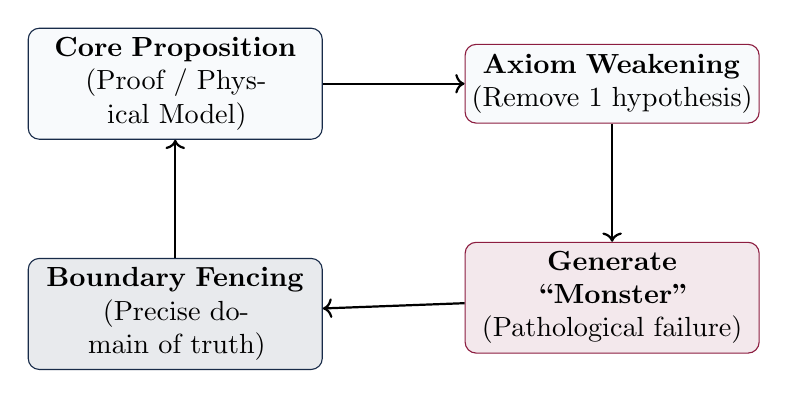
\begin{tikzpicture}[node distance=1.8cm, auto]
    \node [rectangle, draw=primaryblue, fill=boxbg, rounded corners, text width=3.5cm, align=center, minimum height=1cm] (conj) {\textbf{Core Proposition} \\ (Proof / Physical Model)};
    \node [rectangle, draw=accentcrimson, fill=boxbg, rounded corners, text width=3.5cm, align=center, minimum height=1cm, right=1.8cm of conj] (assault) {\textbf{Axiom Weakening} \\ (Remove 1 hypothesis)};
    \node [rectangle, draw=accentcrimson, fill=accentcrimson!10, rounded corners, text width=3.5cm, align=center, minimum height=1cm, below=1.5cm of assault] (monster) {\textbf{Generate ``Monster''} \\ (Pathological failure)};
    \node [rectangle, draw=primaryblue, fill=primaryblue!10, rounded corners, text width=3.5cm, align=center, minimum height=1cm, below=1.5cm of conj] (fence) {\textbf{Boundary Fencing} \\ (Precise domain of truth)};

    \draw [->, thick] (conj) -- (assault);
    \draw [->, thick] (assault) -- (monster);
    \draw [->, thick] (monster) -- (fence);
    \draw [->, thick] (fence) -- (conj);
\end{tikzpicture}
\end{center}

\begin{principlebox}{The Boundary-Assault Drill}
For every major theorem or physical model:
\begin{enumerate}
    \item \textbf{Deconstruct Hypotheses:} List every single condition (e.g., continuity, compactness, linearity, differentiability, boundary at infinity).
    \item \textbf{Violate One Hypothesis:} Remove compactness; set potential $V(x) \to \infty$; allow friction to be velocity-squared; make the metric signature degenerate.
    \item \textbf{Locate the Monster:} Find the exact point where the standard conclusion collapses violently. This defines your true understanding of why the hypothesis was mandatory.
\end{enumerate}
\end{principlebox}

\subsection{Elastic Lossless Compression ($A \xrightarrow{\text{compressed}} E$)}
Your diagram captured \textit{Conceptual Skipping}:
\[
A \longleftrightarrow B \longleftrightarrow C \longleftrightarrow D \longleftrightarrow E \implies A \xrightarrow{\text{compressed}} E
\]

\begin{lawbox}{The Second Law of SIMS: Lossless Compression Verification}
A compressed link $A \to E$ is only valid if it satisfies the \textbf{Bidirectional Decompression Test}:
\begin{equation}
    \text{Compress}(A \dots E) = \mathbf{Key}(A \to E) \quad \text{such that} \quad \mathrm{Decompress}(\mathbf{Key}, \text{Node } C) \equiv C_{\text{exact}}
\end{equation}
Every two weeks, randomly pick one of your ``automated leaps'' ($A \to E$). Forbid yourself from using $E$. Re-derive intermediate node $C$ from scratch using only first principles. If you stumble, the compression was lossy and must be rebuilt.
\end{lawbox}

% =========================================================================
\section{The Dual-Engine Problem-Solving Architecture (70/30)}
% =========================================================================

\subsection{Partitioning the Cognitive Phase Space}
In your notes, problem solving splits into:
\begin{itemize}
    \item \textbf{Path A:} Figuring out, spending significant time, fending the unknown (thinking framework).
    \item \textbf{Path B:} Relating to seen examples (pattern recognition) under time constraints.
\end{itemize}

We formalize this into the \textbf{70/30 Asymmetric Allocation Rule}:

\begin{figure}[h!]
\centering
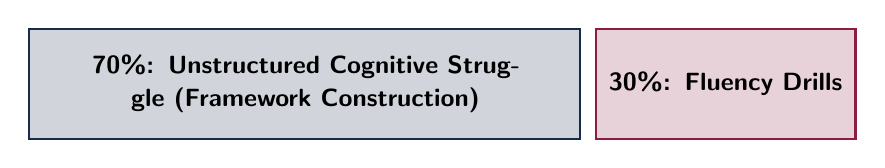
\begin{tikzpicture}
    \draw[fill=primaryblue!20, draw=primaryblue, thick] (0,0) rectangle (7,1.4);
    \node[text width=6.6cm, align=center] at (3.5, 0.7) {\small\bfseries\sffamily 70\%: Unstructured Cognitive Struggle (Framework Construction)};
    
    \draw[fill=accentcrimson!20, draw=accentcrimson, thick] (7.2,0) rectangle (10.5,1.4);
    \node[text width=3.0cm, align=center] at (8.85, 0.7) {\small\bfseries\sffamily 30\%: Fluency Drills};
\end{tikzpicture}
\caption{Cognitive Bandwidth Allocation in the SIMS Framework.}
\end{figure}

\begin{enumerate}
    \item \textbf{The 70\% Exploration Track (Deep Struggle):}
    \begin{itemize}
        \item \textbf{Rules:} No timers. No hint access for a minimum of 45 minutes. Blank unlined paper.
        \item \textbf{Constraint:} You must generate at least \textbf{3 distinct conceptual approaches} before ever looking at a solution.
        \item \textbf{Objective:} Exploring the topography of failure. Even if unsolved, you have mapped 95\% of the dead ends, making the true solution permanently memorable when revealed.
    \end{itemize}
    
    \item \textbf{The 30\% Compilation Track (Algorithmic Muscle Memory):}
    \begin{itemize}
        \item \textbf{Rules:} Strict time limits (e.g., 8--12 minutes per problem). High repetition of standard forms.
        \item \textbf{Objective:} Reduce algebraic cognitive load to absolute zero. When intermediate integrations, tensor contractions, or tactical chess combinations become autonomic, 100\% of working memory is free for high-level strategy.
    \end{itemize}
\end{enumerate}

\subsection{The Variational Re-Derivation Protocol (Banned-Tool Method)}
To solidify Habit \#2 from your notes (\textit{Variation in derivation}):

\begin{principlebox}{The Banned-Tool Protocol}
Never solve a core problem or derive a central theorem using the same paradigm twice. Once derived via the canonical path, deliberately ban your primary tool:
\begin{itemize}
    \item \textbf{Classical Mechanics:} Derive equations of motion using Newtonian vectors. \textit{Banned!} Re-derive via D'Alembert's Principle. \textit{Banned!} Re-derive via Euler-Lagrange. \textit{Banned!} Re-derive via Hamilton's canonical equations or Action-Angle variables.
    \item \textbf{Quantum Mechanics:} Solve the harmonic oscillator via Hermite differential equations. \textit{Banned!} Re-solve using Dirac ladder operators ($a, a^\dagger$). \textit{Banned!} Re-solve using the Feynman path integral.
    \item \textbf{Linear Algebra / Geometry:} Prove spectral decomposition via coordinate matrices. \textit{Banned!} Re-prove using coordinate-free exterior algebra or projective projection operators.
\end{itemize}
\end{principlebox}

% =========================================================================
\section{Cross-Domain Isomorphisms: Physics, Math, Chess, Philosophy}
% =========================================================================

The beauty of the Symmetry-Invariant Metalearning System is that its category-theoretic structure applies universally across all elite intellectual disciplines:

\subsection{Theoretical Physics (Primary Focus)}
\begin{itemize}
    \item \textbf{Dimensional Analysis \& Scaling:} For any equation $f(x, t, m, \hbar, c) = 0$, construct the dimensionless Buckingham-$\pi$ invariants. Analyze behavior under scale transformations $x \to \lambda x$.
    \item \textbf{Asymptotic Extremes:} Always evaluate the 4 physical limits:
    \[
    \lim_{m \to 0}, \quad \lim_{m \to \infty}, \quad \lim_{v \to c} (\text{or } c \to \infty), \quad \lim_{\hbar \to 0}
    \]
    \item \textbf{Variational Action as the Master Functor:} View all fields through the principle of stationary action: $\delta S = \delta \int \mathcal{L} \, d^4x = 0$.
\end{itemize}

\subsection{Pure Mathematics}
\begin{itemize}
    \item \textbf{Definition-Theorem-Proof Decompilation:} Strip away the textbook presentation. Ask: \textit{``What catastrophe would occur if this definition had one less constraint?''}
    \item \textbf{Categorical Duality:} Seek dual objects (e.g., Vectors vs. One-forms, Homology vs. Cohomology, Initial vs. Terminal objects). Solving a problem in the dual category is often trivial.
\end{itemize}

\subsection{Master-Level Chess}
\begin{itemize}
    \item \textbf{Pawn Structure as the Potential Field $V(x)$:} Pawns define the geometric metric of the board. Piece dynamics are simply particles moving through the potential landscape dictated by the pawn skeleton.
    \item \textbf{Kotov Candidate Trees with Pruned Branches:} Formulate 3 candidate moves (System 2 exploration). Run tactical blunder checks (System 1 pattern recognition).
    \item \textbf{Chunking \& Schematic Constellations:} Grandmasters do not calculate 20 moves ahead in all directions; they recognize invariant functional constellations (e.g., ``weak light squares around king'') that compress 8 pieces into 1 conceptual object.
\end{itemize}

\subsection{Philosophy \& Cognitive Psychology}
\begin{itemize}
    \item \textbf{Ontological Primitives:} Break complex philosophical systems into their irreducible ontological primitives (e.g., Spinoza's Substance vs. Kant's Noumena/Phenomena vs. Humean Regularity).
    \item \textbf{Dialectical Synthesis:} Thesis $\oplus$ Antithesis $\implies$ Synthesis. Resolve apparent paradoxes by ascending to a higher-dimensional category where both opposing statements are projections of a single invariant object.
    \item \textbf{Somatic Marker Calibration (Damasio):} In rapid decision-making, pay attention to visceral, bodily signals of error before conscious articulation can justify it.
\end{itemize}

% =========================================================================
\section{The Operational Daily \& Weekly Execution Blueprint}
% =========================================================================

\subsection{The 90-Minute Ultradian Deep Cycle}
Structure each focused theoretical session into the following bio-rhythmic protocol:

\begin{figure}[h!]
\centering
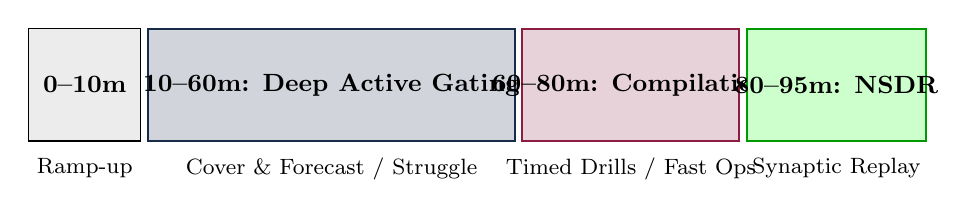
\begin{tikzpicture}[scale=0.95]
    % Phases
    \draw[fill=gray!15, draw=black] (0,0) rectangle (1.5,1.5);
    \node at (0.75,0.75) {\small \textbf{0--10m}};
    \node[below] at (0.75,-0.1) {\footnotesize Ramp-up};

    \draw[fill=primaryblue!20, draw=primaryblue, thick] (1.6,0) rectangle (6.5,1.5);
    \node at (4.05,0.75) {\small \textbf{10--60m: Deep Active Gating}};
    \node[below] at (4.05,-0.1) {\footnotesize Cover \& Forecast / Struggle};

    \draw[fill=accentcrimson!20, draw=accentcrimson, thick] (6.6,0) rectangle (9.5,1.5);
    \node at (8.05,0.75) {\small \textbf{60--80m: Compilation}};
    \node[below] at (8.05,-0.1) {\footnotesize Timed Drills / Fast Ops};

    \draw[fill=green!20, draw=green!60!black, thick] (9.6,0) rectangle (12.0,1.5);
    \node at (10.8,0.75) {\small \textbf{80--95m: NSDR}};
    \node[below] at (10.8,-0.1) {\footnotesize Synaptic Replay};
\end{tikzpicture}
\caption{The 95-Minute Ultradian Neuroplastic Block.}
\end{figure}

\begin{enumerate}
    \item \textbf{Minutes 0--10 (Sensory Ramp-up):} Remove phones and digital distractions completely. Stare at a single fixation point for 60 seconds to mobilize visual acetylcholine. Review the previous session's core invariants.
    \item \textbf{Minutes 10--60 (Deep Active Encoding / 70\% Track):} ``Cover \& Forecast'' active derivation or high-friction problem assault. Welcome cognitive friction as the physical sensation of noradrenaline release.
    \item \textbf{Minutes 60--80 (Compilation / 30\% Track):} Rapid execution drills, automated symbolic manipulation, speed chess tactics, or computational verification.
    \item \textbf{Minutes 80--95 (Non-Sleep Deep Rest / NSDR):} Zero inputs. Eyes closed. No podcasts, no reading. Allow the hippocampus to run high-speed offline replay.
\end{enumerate}

\subsection{The Weekly Variational Matrix}
\begin{table}[h!]
\centering
\small
\begin{tabular}{@{}lll@{}}
\toprule
\textbf{Day} & \textbf{Primary Modality} & \textbf{SIMS Target Objective} \\ \midrule
\textbf{Mon} & Theory Invariant Extraction & Identify Transformation Groups $\mathcal{G}$ and Conserved Core $\mathcal{I}$. \\
\textbf{Tue} & 70\% Deep Struggle & Assault unsolved problems; map failure phase spaces. \\
\textbf{Wed} & 30\% Speed Compilation & Timed problem sets; algebraic muscle memory. \\
\textbf{Thu} & Lakatosian Monster-Barring & Break theorems; construct pathological counterexamples. \\
\textbf{Fri} & Variational Re-Derivation & Re-derive using strictly ``Banned Tools'' (Alternative paths). \\
\textbf{Sat} & Cross-Domain Transfer & Connect physics invariants to pure math, chess, or philosophy. \\
\textbf{Sun} & Lossless Decompression Test & Unpack a compressed $A \to E$ link down to primitive axioms. \\ \bottomrule
\end{tabular}
\caption{The 7-Day Symmetry-Invariant Metalearning Weekly Rhythm.}
\end{table}

\subsection{Summary Formula of the Upgraded System}
In your initial notes, you noted:
\[
\text{Encoding} = \text{Cumulative Exposure Quality} \times \text{Repetition}
\]

We upgrade this to the rigorous \textbf{SIMS Master Equation of Neurocomputational Mastery}:

\begin{equation}
    \mathcal{M} = \int_{0}^{T} \left( \Delta_{\text{PE}}(t) \cdot \Phi_{\text{Invariant}} \cdot \left[ \frac{\mathcal{S}_{\text{struggle}}^{0.7} \cdot \mathcal{C}_{\text{speed}}^{0.3}}{L_{\text{extraneous}}} \right] \right) \cdot e^{-\lambda \cdot \tau_{\text{retrieval}}} \, dt
\end{equation}

Where:
\begin{itemize}
    \item $\Delta_{\text{PE}}$: Prediction error magnitude generated via active forecasting.
    \item $\Phi_{\text{Invariant}}$: Degree of invariant identification (Noetherian grounding).
    \item $\mathcal{S}_{\text{struggle}}$: Depth of unassisted exploratory struggle (70\% track).
    \item $\mathcal{C}_{\text{speed}}$: High-speed algebraic automation (30\% track).
    \item $L_{\text{extraneous}}$: Extraneous cognitive noise (minimized to 1).
    \item $e^{-\lambda \cdot \tau_{\text{retrieval}}}$: Delayed spaced retrieval decay counteracted by variational re-derivation.
\end{itemize}

\end{document}
